\documentclass{beamer}
\usepackage{graphicx}
\newcommand{\quotes}[1]{``#1''}
\graphicspath{ {./images/} }
\mode<presentation>
\title{Properties contaminated with oil - investment scenarios}
\author{Dinkar Ganti}
\begin{document}
\begin{frame}
  \titlepage
\end{frame}
\begin{frame}
\frametitle{Tasks}
\section{Tasks}
  The number of tasks to cleanup a property can spread out over weeks or months and therefore it is important to list them and manage them. Here we list a subset of tasks that need to be caputured in the current real world.
  \begin{itemize}
    \item Baseline analysis or site characterization --- estimated between 5000 - 20000 USD.
    \item Case manager's assessment of the property to provide cleanup guidance.
    \item Environment consultant's cleanup plan.
    \item Environment consultant's rate list as per DEP's desirable rate list per task. 
    \item Installation of cleanup and monitoring equipment.
    \item Liability insurance documents.
  \end{itemize}
\end{frame}
\begin{frame}
\frametitle{TLDR}
\section{TLDR}
  When a release is reported for a property that triggers a set of actions by parties involved due to the liabilities that are ensuant to the release. For example, if the spill is greater than 50 gallons in the state of Virginia, the release is treated as an emergency with a DEP case number assigned. For example,the image shown above describes the closure of a dep case file and the reasons for the closure. More details are outlined in the actual report though, for the purposes of this discussion we the limit our attention to the phrase \quotes{according to state law}, as this encompasses the level of scrutiny each property receives from the relevant DEP (Department of Environment Protection, usually a state regulatory body). The current process is quite labor-intensive and requires a level of effort from many parties including and not limited to the case managers attention to the project plan, the validity of the licenses of the environment contractors, the property owner, the property owner's insurance company and is quite detailed. Each party needs to manage its own part of the project to ensure a timely closure. As we can clearly see that this process needs to be supplemented with a trustless process so that no party has an opportunity to change their mind or data as well as be availble for easy access after a particular task and its associated data have been uploaded on the blockchain.
  
\end{frame}

\begin{frame}
\frametitle{TLDR2}
\section {TLDR2}
  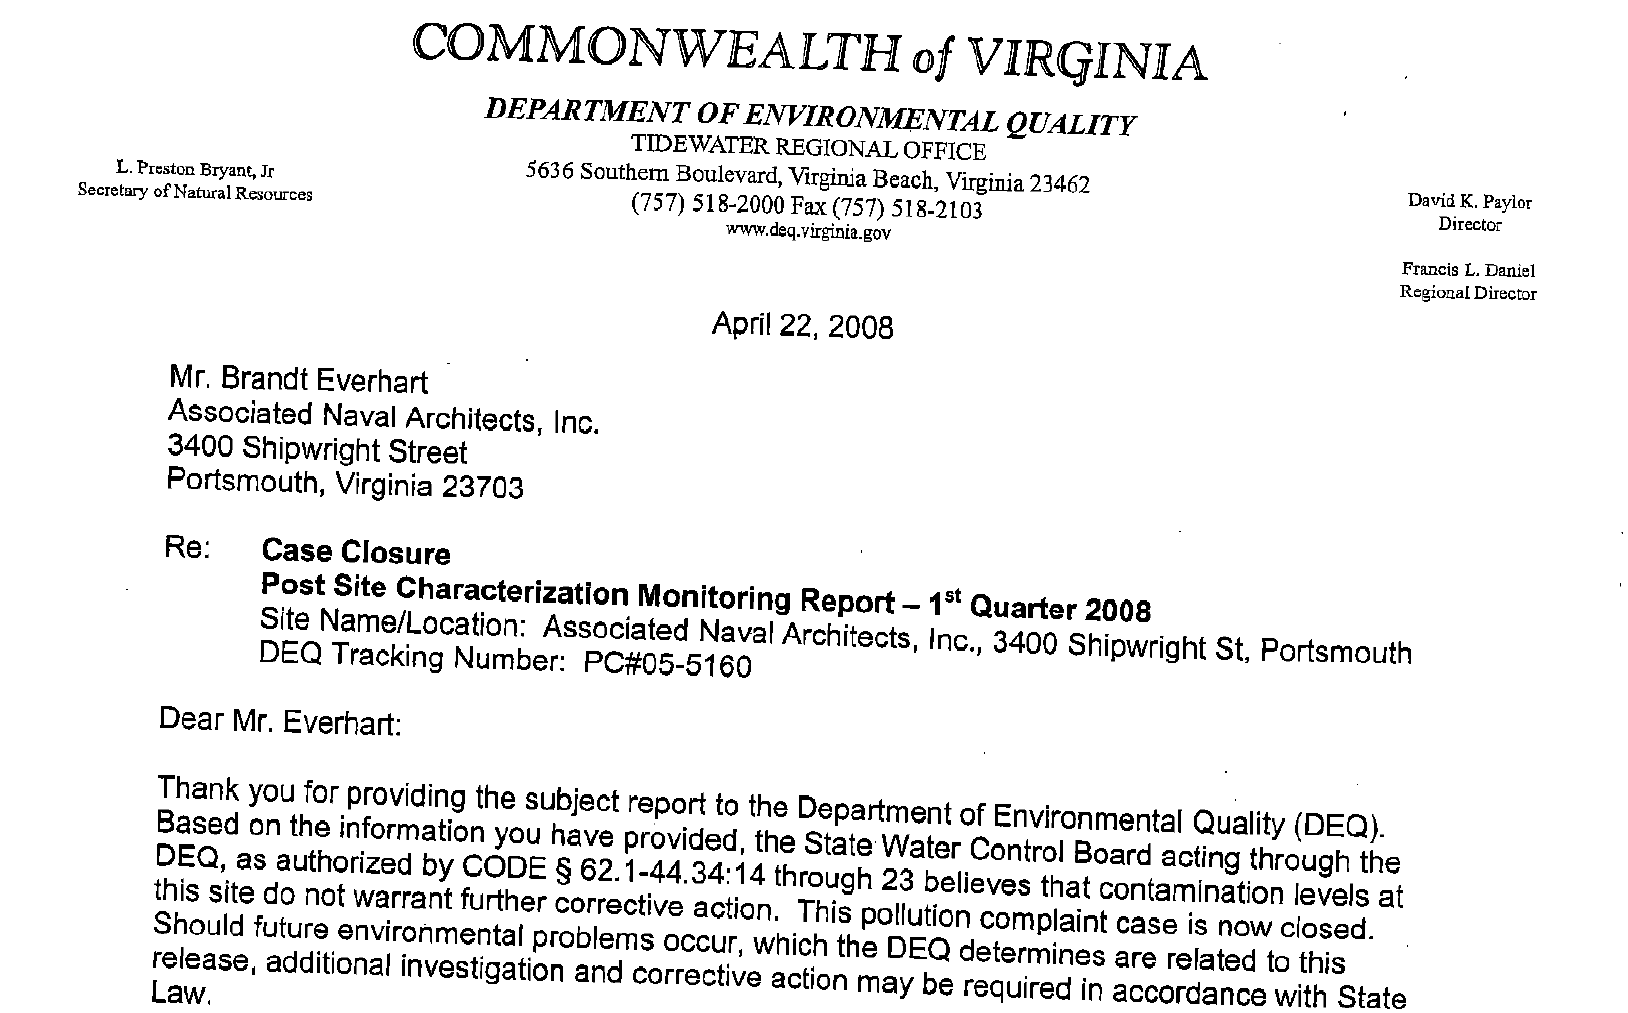
\includegraphics[width = 4in, height = 4in]{vadeqnfa}
\end{frame}
\end{document}